% !TEX program=xelatex
% !Mode:: "TeX:UTF-8"
\documentclass[master,openany,twoside,a4paper,AutoFakeBold]{sudathesis}

% == 内置的package ==
% 添加pdf文件 includepdf命令
\usepackage{pdfpages}
% 全局修改cite为右上角方括号 ;如果使用Overleaf可以注释掉下面2行,使用\upcite() (无自动补全)
\usepackage{natbib}
\setcitestyle{super, square, sort&compress}
% algorithm环境
\usepackage[ruled,linesnumbered]{algorithm2e}
\renewcommand{\algorithmcfname}{算法} % caption部分显示中文名“算法”
% == =========== ==

% == 按需要导入你自己的package ==
\usepackage{graphicx}
\usepackage{float}          % 图表强制位置H
\usepackage{multirow}   % 表格合并单元格
\usepackage{booktabs}  % 表格用于创建漂亮的水平线
\usepackage{stfloats}     % 跨栏图片*/表格*美化
%\usepackage{svg}           % 支持插入矢量图
\usepackage{pifont}        % 勾叉符号
\usepackage{CJKutf8}    % 支持Unicode字符 ├ └ ─
\usepackage[skins]{tcolorbox}  % 文本框
\tcbuselibrary{breakable}% 支持文本框跨页
\usepackage{boites, boites_exemples}
\usepackage{amsmath}
%\usepackage[defaultcolor={red}]{changes}           % 开启修订模式
%\usepackage[final]{changes} % 关闭修订模式
% == ===================== ==

\begin{document}
%\maketitle

% 论文相关信息
% !Mode:: "TeX:UTF-8"

\school
{计算机科学与技术学院}{School of Computer Science and Technology}

% 专业中英文名
\major
{软件工程}{Software Engineering}

% 方向中英文名
\direct
{工具调用}{Tool Learning}

% 论文中英文标题
\thesistitle
{基于xxx的xxx研究}{xxx-based xxx} % 英文题目在sudathesis.cls文件第542行手动修改

% 作者中英文名
\thesisauthor
{学生姓名}{Student Name}

% 导师中英文名
\teacher
{导师姓名}{Mentor Name}


% 班级
\class{自然语言处理1班}

% 学号
\studentID{202242270XX}

% 单位代码
\unicode{10285}

% 论文时间,用于首页
\thesisdate{202X}{6}

% 【PDF】
% 送审版

\includepdf[pages=-]{pdf/DEMO_送审封面.pdf}

% 最终版
%
\includepdf[pages=-]{pdf/DEMO_最终论文封面.pdf}
%
\includepdf[pages=-]{pdf/blank.pdf}
%
\includepdf[pages=-]{pdf/DEMO_独创声明.pdf}
%
\includepdf[pages=-]{pdf/blank.pdf}

% 【摘要】
% 正文前页码是大写罗马字母
\pagenumbering{Roman}
% 前言页眉页脚样式 % 摘要
\pagestyle{cnfrontmatter}
% !Mode:: "TeX:UTF-8"

% 中英文摘要
\begin{cabstract}
	近来出现了许多以带宽换取信噪比的调制方法,比如 PCM 和 PPM,它们的出现进一步激发了人们对广义通信理论的兴趣。在奈奎斯特(Nyquist)和哈特莱(Hartley)发表的一些重要相关论文中,奠定了这一理论的基础。本论文将扩展该理论,增加一些新的因素,具体来说,就是信道中噪声的影响、由于原始消息的统计结构和最终信宿的本质而可能减省的内容。

	通信的基本问题就是在一个地方复现在另一个地方选定的消息,这一复现可能是准确的,也可能是近似的。这些消息通常有特定的含义;也就是说,它们会根据某一系统,与特定的物理或概念实体关联在一起。通信的语义与工程问题无关。重要的是:实际消*是从一个消息集合选出的。所设计的系统必须能够处理任意选定的消息,而不是仅能处理实际选择的特定消息,因为在设计系统时,并不知道会实际选择哪条消息。
	
	如果集合中的消息数目是有限的,而且选择每条消息的可能性相等,那就可以用这个消息数或者它的任意单调函数,来度量从集合中选择一条消息所生成的信息量。正如哈特莱所指出的那样,最自然的选择就是对数函数了。如果考虑消息统计信息的影响,如果消息的选取范围是连续的,那必须对其定义进行重要扩展,但在所有情况下,我们使用的度量在实质上都是对数函数。
	
	——克劳德 E. 香农 1948年 《通信的数学原理》
	\vskip 21bp
	{\heiti\zihao{-4} 关键词:}
	人工智能,
	机器学习,
	物联网,
	边缘计算
	
	\begin{flushright}
		作~~~~~~~~者:XX~~~~XX
		
		指导老师:XXX
		
	\end{flushright}
\end{cabstract}




\pagestyle{enfrontmatter}
% !Mode:: "TeX:UTF-8"

\begin{eabstract}
	THE recent development of various methods of modulation such as PCM and PPM which exchange bandwidth for signal-to-noise ratio has intensified the interest in a general theory of communication. A basis for such a theory is contained in the important papers of Nyquist1 and Hartley2 on this subject. In the present paper we will extend the theory to include a number of new factors, in particular the effect of noise in the channel, and the savings possible due to the statistical structure of the original message and due to the nature of the final destination of the information.

	The fundamental problem of communication is that of reproducing at one point either exactly or approximately a message selected at another point. Frequently the messages have meaning; that is they refer to or are correlated according to some system with certain physical or conceptual entities. These semantic aspects of communication are irrelevant to the engineering problem. The significant aspect is that the actual message is one selected from a set of possible messages. The system must be designed to operate for each possible selection, not just the one which will actually be chosen since this is unknown at the time of design.
	
	If the number of messages in the set is finite then this number or any monotonic function of this number can be regarded as a measure of the information produced when one message is chosen from the set, all choices being equally likely. As was pointed out by Hartley the most natural choice is the logarithmic function. Although this definition must be generalized considerably when we consider the influence of the statistics of the message and when we have a continuous range of messages, we will in all cases use an essentially logarithmic measure.

	A Mathematical Theory of Communication By C. E. SHANNON
	\vskip 21bp
	{\bf\zihao{-4} Key words: }
	Artificial Intelligence,
	Machine Learning,
	Internet of Things,
	Edge Computing
\end{eabstract}

\begin{flushright}
	Written by XXX
	
	Supervised by XXX
\end{flushright}


% 【目录】不设置页眉和页码
\makeatletter
\let \asas \ps@plain
\let \ps@plain \ps@empty
\makeatother
\pagestyle{empty}

% 生成目录
\tableofcontents
\setcounter{secnumdepth}{4}

\makeatletter
\let \ps@plain \asas
\let\asas\relax
\makeatother
\clearpage  %目录3页以上,使用cleardoublepage

% 正文页码样式
\mainmatter
% 正文页眉页脚样式
\pagestyle{mainmatter}
% 正文页码是阿拉伯数字
\pagenumbering{arabic}

% 【 正文】

\chapter{绪论}

\section{研究背景}

对数度量之所以更为便利,其原因有多种:

1. 它在实践中更为有用。一些在工程上非常重要的参数,比如时间、带宽、延迟数,等等,往往与可能性的数量的对数值呈线性关系。例如,增加一个继电器会使继电器的可能状态数加倍。如果对这一数目求以 2 为底的对数,则增加一个继电器后,会使结果加 1。使时间加倍,会使可能消息数近似变为原来的平方,而其对数则是加倍,诸如此类。

2. 它更接近于人类对正确度量的直观认知。这一点与第 1 个原因密切相关,因为人们在对实体进行直觉度量时,通常是与公共标准进行线性比较。比如,人们认为,两张打孔卡存储信息的容量应当是一张打孔卡的两倍,两个相同信道的信息传输能力应当是一个信道的两倍。

3. 更适于数学运算。许多极限运算很容易用对数表示,如果采用可能性的数目表示,可能会需要进行冗繁、笨拙的重新表述。

\section{研究目的与意义}
\subsection{现有解决方法}

\begin{table}
  \centering
  \begin{tabular}{ccc}
    \toprule
    \textbf{文档域类型} & \textbf{Java类型} & \textbf{宽度(字节)} \\
    \midrule
    BOOLEAN  & boolean &  1 \\
    CHAR     & char    &  2 \\
    BYTE     & byte    &  1 \\
    SHORT    & short   &  2 \\
    INT      & int     &  4 \\
    LONG     & long    &  8 \\
    STRING   & String  &  字符串长度 \\
    DATE     & java.util.Date & 8 \\
    BYTE\_ARRAY & byte$[]$ & 数组长度 \\
    BIG\_INTEGER & java.math.BigInteger & 和具体值有关 \\
    BIG\_DECIMAL & java.math.BigDecimal & 和具体值有关 \\
    \bottomrule
  \end{tabular}
  \caption{测试表格}\label{table:test1}
\end{table}


\subsection{现有问题与不足}

测试一下脚注\footnote{测试脚注},测试一下脚注\footnote{测试脚注},测试一下脚
注\footnote{测试脚注},测试一下脚注\footnote{测试脚注},测试一下脚注\footnote{测
  试脚注},测试一下脚注\footnote{测试脚注},测试一下脚注\footnote{测试脚注},测
试一下脚注\footnote{测试脚注},测试一下脚注\footnote{测试脚注},测试一下脚
注\footnote{测试脚注}。

测试一下引用\cite{ACE05}。

下面是一个项目列表:

\begin{itemize}
\item 这是第一项。这是第一项。
\item 这是第二项。这是第二项。
\item 这是第三项。这是第三项。这是第三项。
  \begin{itemize}
  \item 测试第二层列表。测试第二层列表。
  \item 测试第二层列表。测试第二层列表。
  \begin{itemize}
     \item 测试第三层列表。测试第三层列表。
     \item 测试第三层列表。测试第三层列表。
  \end{itemize}
  \end{itemize}
\end{itemize}

下面是一个编号列表:

\begin{enumerate}
\item 这是第一项。这是第一项。这是第一项。这是第一项。这是第一项。这是第一项。这
  是第一项。这是第一项。这是第一项。这是第一项。这是第一项。
\item 这是第二项。这是第二项。
\item 这是第三项。这是第三项。这是第三项。
  \begin{itemize}
  \item 测试第二层列表。测试第二层列表。
  \item 测试第二层列表。测试第二层列表。
  \item 测试第二层列表。测试第二层列表。测试第二层列表。测试第二层列表。测试第二
    层列表。
  \end{itemize}
\item 这是第四项。这是第四项。这是第四项。
  \item 测试第三层列表。测试第三层列表。测试第三层列表。测试第三层列表。测试第三
    层列表。测试第三层列表。
  \item 测试第三层列表。测试第三层列表。
  \item 测试第三层列表。测试第三层列表。测试第三层列表。
\end{enumerate}

\begin{quote}
这是一段引用。这是一段引用。这是一段引用。这是一段引用。这是一段引用。这是一段引用。
这是一段引用。这是一段引用。这是一段引用。这是一段引用。这是一段引用。这是一段引用。
\end{quote}




\subsection{中心观点与思想}

测试一下定理环境。

\begin{algorithm}[] \caption{一般的蒙特卡洛树搜索方法}\label{algo:raw_MCTS} %MCTS
    
    \SetKw{Func}{Function:}
    \SetKw{Return}{Return:}
    
    \Func MCTS($s_0$, $N$)
    
    \KwIn{original state $s_0$, search steps $N$}
    \KwOut{best leaf state $s*$}
    
	 new root node $v_0$ of the tree\; 
	 $v_0$.state $\leftarrow s_0$ \;
	 
	 \While{current search steps $< N$}{
	   $v_l \leftarrow $ tree\_policy($v_0$)\;
	   $\Delta \leftarrow $ default\_policy($v_l$.state)\;
	   backup($v_l, \Delta$)\;
	 } 
	 \Return{$s*$}
\end{algorithm}


\subsection{需要解决的问题与挑战}

测试一下数学公式中的字体大小。

\newcommand{\set}[1]{\left\{\,#1\,\right\}}
\newcommand{\card}[1]{\left|\,#1\,\right|}

Fall-Out指标计算公式如下:
\begin{equation*}
  \mbox{fallout} = \frac{\card{\set{\text{不相关文档}}\cap\set{\text{获取的文档}}}}{\card{\set{\text{不相关文档}}}}
\end{equation*}



\section{研究的应用背景}

\begin{figure}[htbp]
  \centering
  
\includegraphics[width= 0.5\textwidth]{img/SchoolMark.jpg}\\
  \caption{测试插图}\label{fig:test1}
\end{figure}


阿卜·日·法拉兹曾经说过,学问是异常珍贵的东西,从任何源泉吸收都不可耻。带着这句话,我们还要更加慎重的审视这个问题\ref{fig:test1}:它发生了会如何,不发生又会如何。
\chapter{第二章标题}





\chapter{第三章标题}
\chapter{第四章标题}
\chapter{总结与展望}

% % 参考文献,4或者小4楷体
\bibliographystyle{sudathesis}
\addcontentsline{toc}{chapter}{参考文献}
\begin{kai}
    \bibliography{reference}
\end{kai}

% % 附录,4或者小4楷体
% \appendix

% 附页标题样式
\backmatter
% 附页
\pagestyle{backmatter}
\chapter*{攻读学位期间的成果}
\markboth{攻读学位期间的成果}{}
\phantomsection
\addcontentsline{toc}{chapter}{攻读学位期间的成果}
\begin{itemize}
    % \setlength{\itemsep}{5pt}
	 \setlength{\parsep}{2em}
	\item \textbf{\heiti\sihao{论文}}
	      \begin{enumerate}
	      	\setlength{\itemsep}{-\itemsep}  %调整间距
	      	% \usecounter{numcount} % 使用计数器,初始值为0
	      	% \setlength{\leftmargin}{3em} %左边界
	      	% \setlength{\parsep}{-0.5ex} %段落间距
	      	% \setlength{\topsep}{-10ex} %列表到上下文的垂直距离
	      	% \setlength{\itemsep}{0.5ex} %条目间距
	      	% \setlength{\labelsep}{0.3em} %标号和列表项之间的距离,默认0.5em
	      	% \setlength{\itemindent}{1.1em} %标签缩进量
	      	% \setlength{\listparindent}{0em} %段落缩进量
	      	
	      	      
        \item \textbf{Wu, M.}, Zhu, T., Han, H., Tan, C., Zhang, X., Chen, W. (2025). \emph{Seal-Tools: Self-instruct Tool Learning Dataset for Agent Tuning and Detailed Benchmark}. In: Wong, D.F., Wei, Z., Yang, M. (eds) Natural Language Processing and Chinese Computing. NLPCC 2024. Lecture Notes in Computer Science(), vol 15360. Springer, Singapore. https://doi.org/10.1007/978-981-97-9434-8\_29
        \item \textbf{Mengsong Wu}, Tong Zhu, Guoliang Zhang, Junfei Ren, Zijian Yu and Wenliang Chen. \emph{A Document-Level Event Extraction Model for Chinese Table-Text Mixed Documents}. CCKS2023.
        \item \textbf{Mengsong Wu}, Tong Zhu, Han Han, Xiang Zhang, Wenbiao Shao and Wenliang Chen. \emph{Chain-of-Tools: Utilizing Massive Unseen Tools in the CoT Reasoning of Frozen Language Models}.
        \item \textbf{Mengsong Wu}, Di Zhang, Yuqiang Li, Dongzhan Zhou, Wenliang Chen. \emph{SELT: Self-Evaluation Tree Search for LLMs with Task Decomposition}.
        \item \textbf{Mengsong Wu}, YaFei Wang, Di Zhang, Yidong Ming, Yuqi An, Yuwei Wan, Wenliang Chen, etal. \emph{ChemAgent: Enhancing LLMs for Chemistry and Materials Science through Tree-Search Based Tool Learning}.
	      	      
	      \end{enumerate}
	      
 		\item \textbf{\heiti\sihao{实习}}
	      \begin{enumerate}
	      	\item 
	      \end{enumerate}
	      
		\item \textbf{\heiti\sihao{比赛}}
	      \begin{enumerate}
	      	\item 
	      \end{enumerate}

\end{itemize}


\pagestyle{thankmatter}
\chapter*{致谢}
\markboth{致谢}{}
\phantomsection
\addcontentsline{toc}{chapter}{致谢}


\includepdf[pages=-]{pdf/blank.pdf}
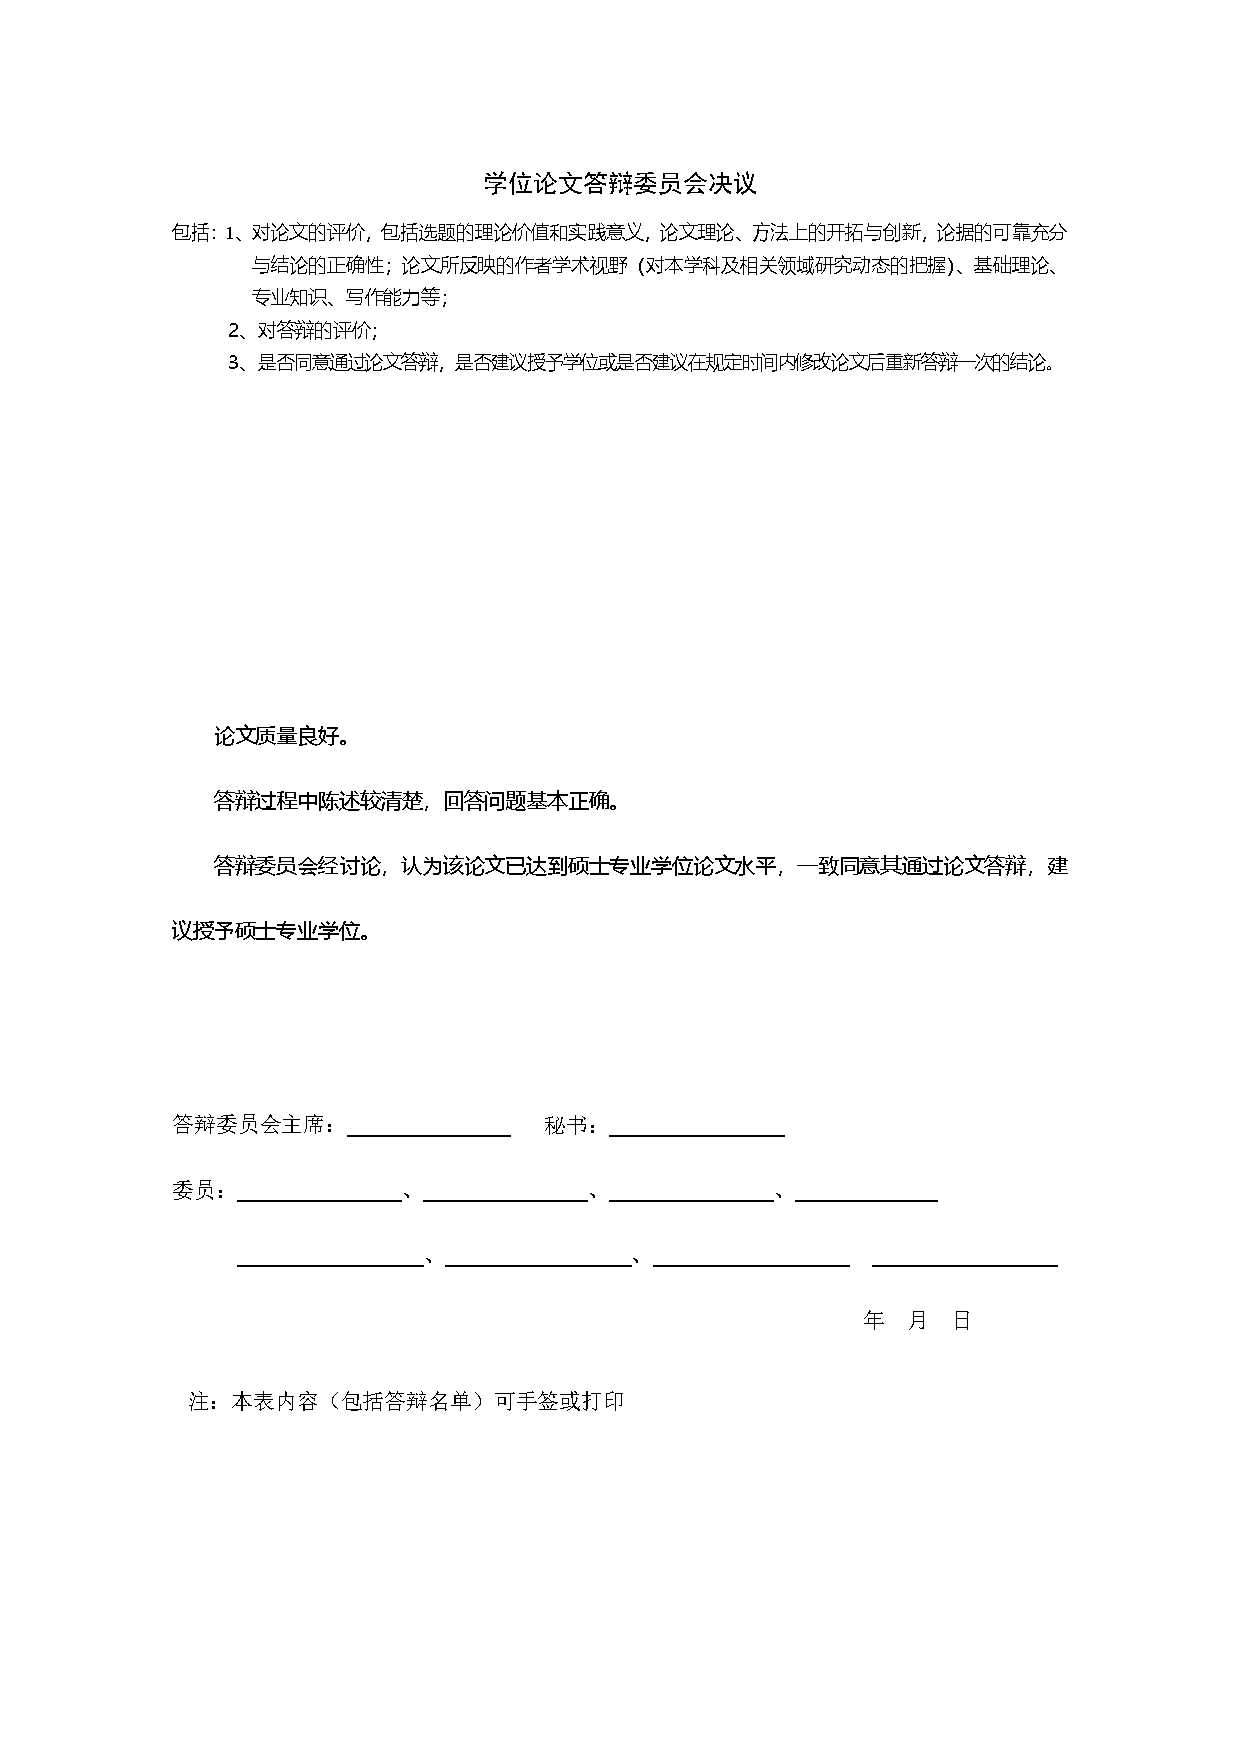
\includepdf[pages=-]{pdf/DEMO_答辩决议书.pdf}

\end{document}